\documentclass[
  bibliography=totoc,     % Literatur im Inhaltsverzeichnis
  captions=tableheading,  % Tabellenüberschriften
  titlepage=firstiscover, % Titelseite ist Deckblatt
]{scrartcl}
\usepackage{parskip}
% Paket float verbessern
\usepackage{scrhack}

% Warnung, falls nochmal kompiliert werden muss
\usepackage[aux]{rerunfilecheck}

% deutsche Spracheinstellungen
\usepackage{polyglossia}
\setmainlanguage{german}

% unverzichtbare Mathe-Befehle
\usepackage{amsmath}
% viele Mathe-Symbole
\usepackage{amssymb}
% Erweiterungen für amsmath
\usepackage{mathtools}

% Fonteinstellungen
\usepackage{fontspec}
% Latin Modern Fonts werden automatisch geladen

\usepackage[
  math-style=ISO,    % ┐
  bold-style=ISO,    % │
  sans-style=italic, % │ ISO-Standard folgen
  nabla=upright,     % │
  partial=upright,   % ┘
  warnings-off={           % ┐
    mathtools-colon,       % │ unnötige Warnungen ausschalten
    mathtools-overbracket, % │
  },                       % ┘
]{unicode-math}

% traditionelle Fonts für Mathematik
\setmathfont{Latin Modern Math}
\setmathfont{XITS Math}[range={scr, bfscr}]
\setmathfont{XITS Math}[range={cal, bfcal}, StylisticSet=1]

% Zahlen und Einheiten
\usepackage[
  locale=DE,                 % deutsche Einstellungen
  separate-uncertainty=true, % immer Fehler mit \pm
  per-mode=reciprocal,       % ^-1 für inverse Einheiten
  %output-decimal-marker=.,   % . statt , für Dezimalzahlen
]{siunitx}

% chemische Formeln
\usepackage[
  version=4,
  math-greek=default, % ┐ mit unicode-math zusammenarbeiten
  text-greek=default, % ┘
]{mhchem}

% richtige Anführungszeichen
\usepackage[autostyle]{csquotes}

% schöne Brüche im Text
\usepackage{xfrac}

% Standardplatzierung für Floats einstellen
\usepackage{float}
\floatplacement{figure}{htbp}
\floatplacement{table}{htbp}

% Floats innerhalb einer Section halten
\usepackage[
  section, % Floats innerhalb der Section halten
  below,   % unterhalb der Section aber auf der selben Seite ist ok
]{placeins}

% Seite drehen für breite Tabellen
\usepackage{pdflscape}

% Captions schöner machen.
\usepackage[
  labelfont=bf,        % Tabelle x: Abbildung y: ist jetzt fett
  font=small,          % Schrift etwas kleiner als Dokument
  width=0.9\textwidth, % maximale Breite einer Caption schmaler
]{caption}
% subfigure, subtable, subref
\usepackage{subcaption}

% Grafiken können eingebunden werden
\usepackage{graphicx}
% größere Variation von Dateinamen möglich
\usepackage{grffile}

% schöne Tabellen
\usepackage{booktabs}

% Verbesserungen am Schriftbild
\usepackage{microtype}

% Literaturverzeichnis
\usepackage[
  style=numeric,
  sorting=none,
  backend=biber,
]{biblatex}
% Quellendatenbank
\addbibresource{lit.bib}
\addbibresource{programme.bib}

%Biber bringt nichts durcheinander
%\usepackage[sort&compress,numbers]{natbib}

% Hyperlinks im Dokument
\usepackage[
  unicode,        % Unicode in PDF-Attributen erlauben
  pdfusetitle,    % Titel, Autoren und Datum als PDF-Attribute
  pdfcreator={},  % ┐ PDF-Attribute säubern
  pdfproducer={}, % ┘
]{hyperref}
\hypersetup{breaklinks=true,
            bookmarks=true,
            colorlinks=true,
            citecolor=blue,
            urlcolor=blue,
            linkcolor=red,
            pdfborder={0 0 0}
            }
% erweiterte Bookmarks im PDF
\usepackage{bookmark}

% Trennung von Wörtern mit Strichen
\usepackage[shortcuts]{extdash}

% tikzpicture
\usepackage{tikz}
\usetikzlibrary{circuits.ee.IEC}
\usetikzlibrary{positioning}
\tikzset{
  Pfeil/.style={thick,shorten >=#1,shorten <=#1,->,>=latex}, % für Peile
  UPfeil/.style={blue,Pfeil=#1,font={\sffamily\itshape}},% für Spannungspfeile
  IPfeil/.style={red,Pfeil=#1,font={\ttfamily\itshape}} % für Strompfeile
}
%Volt- und Amperemeter festlegen:
\tikzset{circuit declare symbol = Us}
\tikzset{set Us graphic ={draw,generic circle IEC, minimum size=5mm,info=center:$U_s$}}

\tikzset{circuit declare symbol = voltmeter}
\tikzset{set voltmeter graphic ={draw,generic circle IEC, minimum size=5mm,info=center:V}}


\author{
  Johannes Kollek%
  \texorpdfstring{
    \\
    \href{mailto:johannes.kollek@udo.edu}{johannes.kollek@udo.edu}
  }{}%
  \texorpdfstring{\and}{, }
  Jean-Marco Alameddine%
  \texorpdfstring{
    \\
    \href{mailto:jean-marco.alameddine@udo.edu}{jean-marco.alameddine@udo.edu}
  }{}%
}
\publishers{TU Dortmund – Fakultät Physik}


\subject{Versuchsprotokoll zum Versuch US1}
\title{Grundlagen der Ultraschalltechnik}
\date{
  Durchführung: 03.05.2016
}

\begin{document}

\maketitle
\thispagestyle{empty}
\tableofcontents
\newpage

\section{Theorie}
\label{sec:Theorie}

\cite{sample}

\clearpage
\newpage
\section{Fehlerrechnung}
Im folgenden Kapitel werden die wichtigsten Formeln der Fehlerrechnung aufgelistet, welche für die folgende Versuchsauswertung benötigt werden.
Der Mittelwert $\overline{x}$ einer Messgröße $x$ bei einer Gesamtanzahl von $N$ Messungen berechnet sich zu
\begin{equation}
  \label{eq:std}
  \overline{x} = \frac{1}{N} \sum_{i=1}^Nx_i.
\end{equation}
Der Fehler des Mittelwertes berechnet sich zu
\begin{equation}
  \label{eq:std_mean}
  \Delta \overline{x} = \sqrt{\frac{1}{N(N-1)}\sum_{i=1}^N(x_i-\overline{x})^2}   \; .
\end{equation}
%Die Schätzung der Standardabweichung berechnet sich zu
%\begin{equation}
%  \label{eq:std}
%  \Delta x = \sqrt{\frac{1}{N-1}\sum_{i=1}^N(x_i-\overline{x})^2}     \; .
%\end{equation}

Für die Fehlerrechnung wird bei allen folgenden Rechnungen das Gaußsche Fehlerfortpflanzungsgesetz
\begin{equation}
\increment{f} = \sqrt{\Bigl(\frac{\partial f}{\partial x_1}\increment{x_1}\Bigr)^2 + \Bigl(\frac{\partial f}{\partial x_2}\increment{x_2}\Bigr)^2 + \dotsc + \Bigl(\frac{\partial f}{\partial x_n}\increment{x_n}\Bigr)^2} \label{gauss}
\end{equation}
für eine Funktion $f(x_1,x_2, \dotsc ,x_n)$, bei der die Größen $x_1, x_2, \dotsc , x_n$ mit ihren Ungenauigkeiten $ \increment{x_1}, \increment{x_2}, \dotsc , \increment{x_n}$ voneinander unabhängig sind, verwendet.

%Bei der linearen Regressionsrechnung gilt mit den Parametern $m$ und $b$ und der Ausgleichsgerade $y=mx+b$ der Zusammenhang:
%\begin{align}
%  m &= \frac{\overline{xy}-\overline{x}\cdot\overline{y}}{\overline{x²} - \overline{x}²} & &  b = \overline{y} - m \overline{x}  \; .
%\end{align}
%Dabei sind $x_i$ und $y_i$ linear abhängige Messgrößen. Der Fehler dieser Parameter errechnet sich zudem zu
%\begin{align}
%  \sigma_m^2 &= \frac{\sigma^2}{n(\overline{x²} - \overline{x}²)} & &\sigma_b^2 = \frac{\sigma^2\overline{x²}}{n(\overline{x²} - \overline{x}²)}
%\end{align}
% Wenn Messdaten mit Vorhersagen verglichen werden sollen, benutzt man häufig die \emph{root mean square deviation}. Diese ist gegeben durch
% \begin{equation}
%   \label{eq:RMSE}
%   \textrm{RMSD} = \sqrt{\overline{(Y_\textrm{Messung}-Y_\textrm{Vorhersage})^2}}  \; .
% \end{equation}

\clearpage
\newpage
\section{Aufbau und Durchführung}
\subsection{Aufbau}
\label{sec:Aufbau}

Das im vorliegenden Versuch verwendete Michelson-Interferometer ist in Abbildung \ref{abb:2} schematisch dargestellt.
\begin{figure}[H]
  \centering
  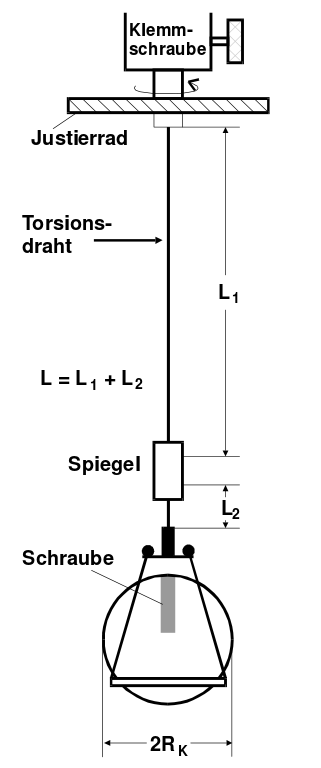
\includegraphics[height=4cm]{ressources/aufbau1.png}
  \caption{Schematischer Aufbau eines Michelson Interferometers. cite{skript2}}
  \label{abb:2}
\end{figure}

\subsubsection{Grundlegender Aufbau der Michelson-Interferometers}
Ein Lichtstrahl, welcher hier durch einen Laser erzeugt wird, wird vom Ort $L$ zu einem halbdurchlässigen Spiegel am Ort $P$ gelenkt.
Durch die Eigenschaften des halbdurchlässigen Spiegels wird der Strahl nun entweder zum Spiegel $S_1$ reflektiert oder zum Spiegel $S_2$ durchgelassen.
Beide Strahlen werden nun am jeweiligen Spiegel reflektiert, der erste Strahl kann nun wieder eine Reflexion an $P$ erfahren oder durchgelassen werden: In diesem Fall endet der Lichtstrahl am Detektor $D$.
Beim zweiten Strahl, der vom Spiegel $S_2$ kommt, können ebenfalls beide Fälle auftreten.
Im Falle einer Reflexion jedoch tritt nun eine Phasenverschiebung von $\frac{\lambda}{2}$ auf und der Strahl endet am Detektor.
Da der eine Strahl dreimal den semipermeablen Spiegel durchläuft und der andere nur einmal treten Abweichungen auf.
Diese werden beseitigt, indem eine Kompensationsplatte mit den gleichen Maßen wie der halbdurchlässige Spiegel $P$ in den Strahlengang von $S_2$ gesetzt wird.
Durch diesen Aufbau wird gewährleistet, dass bei einem identischen Abstand von $P$ zu $S_1$ und $S_2$ eine Phasendifferenz der beiden am Detektor ankommenden Strahlen von $\frac{\lambda}{2}$ besteht.
Dieser Phasenunterschied kann nun auf verschiedene Weisen beeinflusst werden.

\subsubsection{Variation der Spiegelabstände}
Die erste Möglichkeit die Wegdifferenz der Strahlen zu variieren, ist die Verschiebung einer der Platten.
Dies geschieht mit einem Synchronmotor, welcher über einen Untersetzungshebel den Abstand der Spiegel genau variieren kann.
Das exakte Ablesen der Streckendifferenz erfolgt über eine Mikrometerschraube.
Der Synchronmotor kann auf verschiedene Geschwindigkeiten eingestellt werden, so dass die Variationsgeschwindigkeit des Abstandes geregelt werden kann.

\subsubsection{Variation des Mediums}
Eine weitere Möglichkeit zur Erzeugung einer Phasenverschiebung ist das Verändern des Mediums in einem der Strahlengänge.
Hierbei erfährt der Lichtstrahl nach Formel \eqref{eqn:3} eine optische Weglängenänderung.
Hierzu wird eine Messzelle der Dicke $b$ verwendet, bei der sowohl der Druck als auch das Medium an sich variiert werden kann.

\subsubsection{Detektion der Interferenzeffekte}
Zur Detektion der Interferenzeffekte wird ein Photoelement verwendet, welches eintreffendes Licht als Impuls wahrnimmt.
Zum Zählen der in einem Zeitraum auftretenden Maxima und Minima wird dieses Signal verstärkt und in einem elektronischen Zählwerk ausgewertet.

\clearpage
\newpage
\section{Durchführung}
\label{sec:Durchführung}
%\subsection{Aufbau}
%Die Schwebungen werden mit einem Schwingkreis, wie in Abbildung \ref{fig:1}, untersucht.








\subsection{Justierungen}
\label{sec:d0}
Die Schwebungen werden mit einem Schwingkreis, wie in Abbildung \ref{fig:schwingkreis} aus der Theorie, untersucht.
Bevor die Messreihen beginnen, müssen gewisse Justierungen getroffen werden.
Um, wie in der Theorie beschrieben, einen möglichst guten Energieaustausch zu gewährleisten, sollten die beiden Schwingkreise die selbe Resonanzfrequenz besitzen.
Dazu wird zuerst die Schaltung aus Abbildung \ref{fig:2} nachgebaut.

\begin{figure}[H]
  \centering
  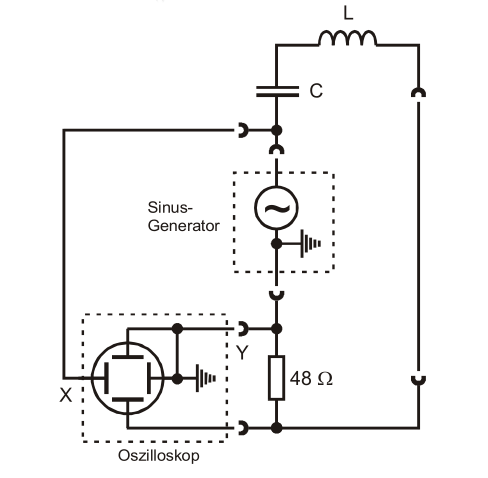
\includegraphics[height=6cm]{just1.png}
  \caption{linke Masche. \cite{sample}}
  \label{fig:2}
\end{figure}

Sie besteht aus einem Sinusgenerator und jeweils dazu einen in Reihe geschalteten Kondensator und einer Spule.
Ein Oszilloskop misst nach der Spule an einem Ohmschen Widerstand die Spannung über den Y-Eingang.
Dessen X-Eingang wird zwischen Generator und Kondensator zugesteckt.
Sie repräsentiert die linke Masche des gesamten Schwingkreises, wobei der Kondensator $C_k$ überbrückt wird.\\
Eine Resonanz liegt vor wenn die Phase zwischen Generatorspannung und Schwingkreisstrom 0 beziehungsweise $\pi$ ist.
Dies wird über die Lissajous-Figur über das Oszilloskop bestimmt.
Nun wird die Frequenz der Sinusspannung solange variiert, bis die Resonanz des Schwingkreises beobachtet wird.
Die Frequenz wird vermerkt.
Als nächstes wird die rechte Seite des gesamten Schwingkreises aufgebaut, die in Abbildung \ref{fig:3} dargestellt wird.

\begin{figure}[H]
  \centering
  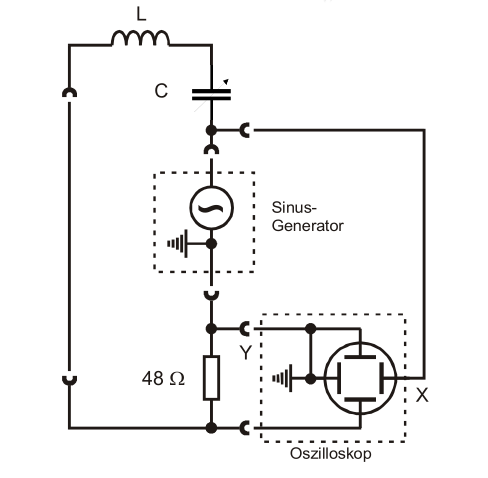
\includegraphics[height=6cm]{just2.png}
  \caption{rechte Masche.}
  \label{fig:3}
\end{figure}

Es befindet sich jedoch an Stelle eines festen ein regelbarer Kondensator in der Schaltung.\\
Dieser Schwingkreis wird nun mit der Resonanzfrequenz des linken betrieben.
Hierbei wird jedoch die Kapazität des Kondensators variiert, bis erneut eine Resonanz erzeugt wird.
Die beiden Maschen haben nun die selbe Resonanzfrequenz und sind somit aufeinander abgestimmt.
Die Messreihe kann nun beginnen.\\
\subsection{Bestimmung der Schwebungsfrequenzen}
\label{sec:d1}
Nun wird der gesamte Aufbau betrachtet.
Die beiden Maschen werden über den gemeinsamen, nun zugeschalteten Koppelkondensator $C_k$ miteinander verbunden.
Der Generator liegt nun wieder an der linken Masche an.
Die Abbildung \ref{fig:4} realisiert dies.

\begin{figure}[H]
  \centering
  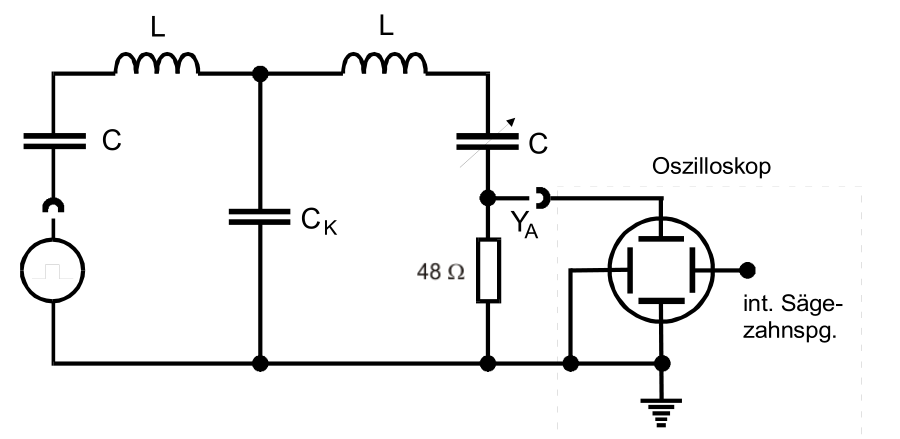
\includegraphics[height=6cm]{a.png}
  \caption{1. Messreihe. \cite{sample}}
  \label{fig:4}
\end{figure}

Der linke Schwingkreis wird extern mittels Rechtecksignal zum Schwingen angeregt.
Auf dem Oszilloskop können die Schwebungen beobachtet werden.
Die Maxima innerhalb einer Schwebung werden notiert.
An ihnen kann das Verhältnis zwischen Schwingungs- und Schwebungsfrequenz abgelesen werden.
Die Messreihe kommt zustande, indem $C_k$ in einem bestimmten Bereich variiert wird.\\
\subsection{Bestimmung der Fundamentalfrequenzen}
\label{sec:d2}
Als Nächstes werden die Frequenzen der Fundamentalschwingung in Abhängigkeit der Kapazität des Koppelkondensators $C_k$ gemessen.
Hierzu wird die Schaltung aus Abbildung \ref{fig:5} nachgebaut.

\begin{figure}[H]
  \centering
  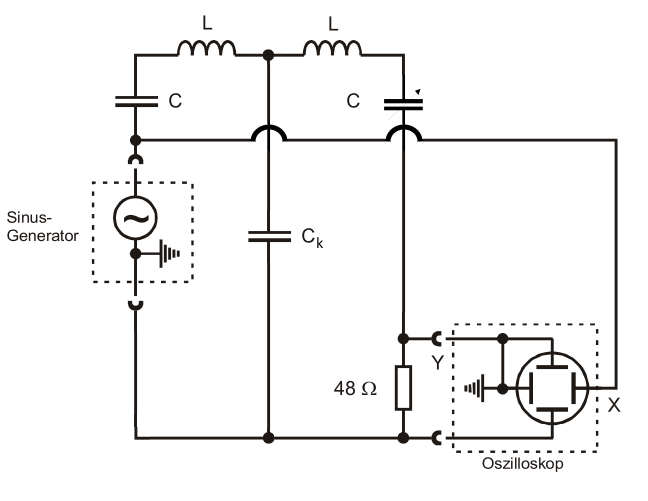
\includegraphics[height=6cm]{b.png}
  \caption{2. und 3. Messreihe.}
  \label{fig:5}
\end{figure}

Der Generator führt dem Stromkreis wieder eine Sinusspannung zu, die von dem X-Eingang des Oszilloskops abgegriffen wird.
Jetzt wird über die Lissajous-Figur die Resonanzfrequenz ermittelt.
Dies wird wider für verschiedene $C_k$ wiederholt.\\
\subsection{Bestimmung eines Frequenzspektrums}
\label{sec:d3}
Zuletzt soll der Verlauf der beiden Ströme $I_2$ und $I_k$ untersucht werden.
Dazu wird der selbe Aufbau wie zuvor, dargestellt in Abbildung \ref{fig:5}, verwendet.
Nun wird jedoch ein Frequenzspektrum durchlaufen.
Auf dem Oszilloskop erscheinen dementsprechend die beiden Resonanzpeaks in Abhängigkeit von der Zeit.
Die Zeiten von der Startfrequenz bis zum Erreichen der Peaks wird notiert.
Dies wird wie zuvor für verschiedene $C_k$ wiederholt.

\clearpage
\newpage
\section{Auswertung}
\label{sec:Auswertung}

\subsection{Bestimmung einer Ausgleichskurve}
\begin{figure}
  \centering
  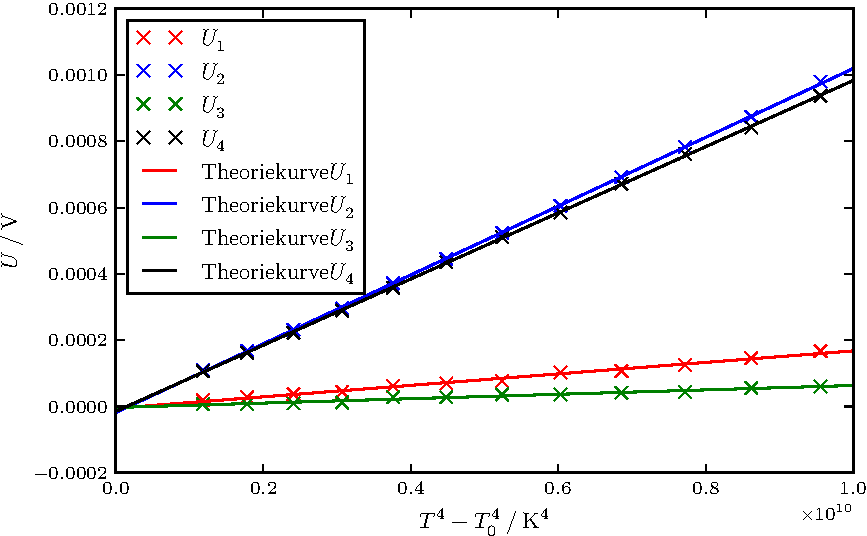
\includegraphics{plot.pdf}
  \caption{Plot.}
  \label{fig:plot}
\end{figure}
Die gemessenen Daten für die Tempeatur $T_1$ des wärmeren sowie die Temperatur
$T_2$ des kälteren Reservoirs wurden gegen die Zeit $t$ in Minuten abgetragen.
Mithilfe von SciPy wurde jeweils eine Ausgleichskurve für die folgende Funktion
berechnet:
\begin{equation}
  T(t)=A \cdot t^2 + B \cdot t + C
\end{equation}
Die Parameter $A$, $B$ und $C$ wurden bestimmt zu
\begin{align*}
A_{T_1} &= \SI{-3.87601 +- 0.10382e-6}{\kelvin\per\second²} \\
B_{T_1} &= \phantom{1}\SI{0.02345 +- 0.00019}{\kelvin\per\second} \\
C_{T_1} &= \phantom{1}\SI{293.592 +- 0.062}{\kelvin} \\
A_{T_2} &= \phantom{1}\SI{4.34879 +- 0.08533e-6}{\kelvin\per\second²}  \\
 B_{T_2} &= \SI{-0.01815 +- 0.00016}{\kelvin\per\second} \\
  C_{T_2} &= \phantom{1}\SI{294.936 +- 0.062}{\kelvin}
\end{align*}

Durch Ableiten und Einsetzen in die Ausgleichskurve
\begin{equation}
  \frac{\symup{d}T}{\symup{d}t}= 2 \cdot A \cdot t + B
\end{equation}
erhält man folgende Werte der Differentialquotienten:
\begin{table}
  \centering
  \caption{Differentialquotienten}
  \label{tab:tabelle1}
  \sisetup{table-format=1.2}
  \begin{tabular}{c c c c c}
    \toprule
    {$t [\si{\second}]$} & {$T_1 [\si{\kelvin}]$} & {$T_2 [\si{\kelvin}]$} & {$\frac{\symup{d}T_1}{\symup{d}t} [\si{\kelvin\per\second}]$}  & {$\frac{\symup{d}T_2}{\symup{d}t} [\si{\kelvin\per\second}]$}\\
    \midrule
    \num{420} & \num{29.6 +- 0.1} & \num{14.9 +- 0.1} & \num{0.021954 +- 0.000212} & \num{-0.014500 +- 0.000174} \\
    \num{840} & \num{37.5 +- 0.1} & \num{19.5 +- 0.1} & \num{0.016940 +- 0.000260} & \num{-0.010846 +- 0.000214} \\
    \num{1260} & \num{43.7 +- 0.1} & \num{5.7 +- 0.1} & \num{0.013684 +- 0.000325} & \num{-0.007193 +- 0.000267} \\
    \num{1680} & \num{48.9 +- 0.1} & \num{3.5 +- 0.1} & \num{0.010428 +- 0.000399} & \num{-0.003988 +- 0.000328} \\
    \bottomrule
  \end{tabular}
\end{table}
\\
Für die Fehlerrechnung wurde bei der vorliegenden Rechnung und bei allen folgenden Rechnungen das Gauß\'sche Fehlerfortpflanzungsgesetz
\begin{equation}
\increment{f} = \sqrt{(\frac{\partial f}{\partial x_1}\increment{x_1})^2 + (\frac{\partial f}{\partial x_2}\increment{x_2})^2 + \dotsc + (\frac{\partial f}{\partial x_n}\increment{x_n})^2}
\end{equation}
für eine Funktion $f(x_1,x_2, \dotsc ,x_n)$ bei denen die Größen $x_1, x_2, \dotsc , x_n$ voneinander unabhängig sind.

\subsection{Güteziffervergleich}
Für eine ideale Wärmepumpe gilt
\begin{equation}
  v_{ideal} = \frac{T_1}{T_1-T_2}.
\end{equation}
Für die reale Wärmepunpe gilt jedoch die Formel
\begin{equation}
  v_{real}= \frac{\symup{d} Q_1}{\symup{d} tN} = (m_1c_w+m_kc_k)\frac{\symup{d} T_1}{\symup{d} tN}.
\end{equation}
wobei $ N = $ die Kompressorleistung, $ m_1$ die Masse des Wassers in $ R_1 $, $m_k$ die Masse des zu heizenden Reservoirs inklusive Kupferrohre, $ c_w $ die spezifische Wärmekapazität des Wassers sowie $ c_k $ die spezifische Wärmekapazität des Reservoirs und der Kuperrohre ist.
Da bei der Durchführung des Versuches \SI{4}{\litre} Wasser für $R_1$ verwendet wurden, berechnet sich $m_1$ zu $m_1 = \rho_{H_2O} \cdot V = \SI{4176.48}{\kilogram}$, wobei der Werte für $\rho_{H_20}$ der Literatur entnommen wurde.
Das Produkt aus $m_k$ und $c_k$ wurde vom Versuchsaufbau zu $\SI{750}{\joule\per\kelvin}$ abgelesen, $c_w$ wurde ebenfalls der Literatur zu $\SI{4,1819}{\kilo\joule\per\kilogram\kelvin}$ entnommen.
Die Kompressorleistung ergibt sich aus dem arithmetischen Mittelwert der Messdaten zu $N=124.77$.
Für die Differenzenquotienten wurden die Werte der Ausgleichskurve, angegeben in Tabelle 1 verwendet.

\begin{table}
  \centering
  \caption{Güteziffervergleich}
  \label{tab:tabelle1}
  \sisetup{table-format=1.2}
\begin{tabular}{c c c c c c c}
  \toprule
  {$t [\si{\second}]$} & {$T_1 [\si{\kelvin}]$} & {$T_2 [\si{\kelvin}]$} & {$\increment{T} [\si{\kelvin}]$} & {$v_{real, T_1}$}  & {$v_{real, T_2}$} & {$v_{ideal}$}\\
  \midrule
  \num{420} & \num{29.6 +- 0.1} & \num{14.9 +- 0.1} & \num{14.7 +- 0.1} & \num{2.948 +- 0.039} & \num{-2.117 +- 0.031} & \num{20.599 +- 0.193} \\
  \num{840} & \num{37.5 +- 0.1} & \num{19.5 +- 0.1} & \num{18.0 +- 0.1} & \num{2.473 +- 0.043} & \num{-1.584 +- 0.034} & \num{11.096 +- 0.054}  \\
  \num{1260} & \num{43.7 +- 0.1} & \num{5.7 +- 0.1} & \num{38.0 +- 0.1} & \num{1.998 +- 0.050} & \num{-1.050 +- 0.040} & \num{8.339 +- 0.029}  \\
  \num{1680} & \num{48.9 +- 0.1} & \num{3.5 +- 0.1} & \num{45.4 +- 0.1} & \num{1.522 +- 0.059} & \num{-0.517 +- 0.048} & \num{7.095 +- 0.021}  \\
  \bottomrule
\end{tabular}
\end{table}
Es fällt auf, dass sich die reale Güteziffer deutlich von der idealen Güteziffer unterscheidet.
Gründe für diese Differenz werden im Kapitel Diskussion besprochen.
\subsection{Massendurchsatz}

\clearpage
\newpage
\section{Diskussion}
\label{sec:Diskussion}
Bei Mehrelektronenatomen wird die Kernladung durch die Elektronen
abgeschirmt, sodass die Elektronen in den äußeren Schalen eine geringere
Bindungsenergie besitzen als in den inneren Schalen und somit leichter
herausgeschlagen werden können. Durch Bestimmung der K-Kanten kann
mithilfe von Formel \eqref{eq:sigma_k} die Abschirmzahl
$\sigma_\mathrm{K}$ bestimmt werden. Dabei bezeichnet $\alpha$ die
Feinstrukturkonstante, $Z$ die Kernladungszahl $E_\text{K}$ die Energie
der K-Kante und $R_\infty$ die Rydberg-Konstante.
%
\begin{equation}
  \sigma_\text{K} = Z - \sqrt{\frac{E_\text{K}}{h c R_\infty}
    - \frac{\alpha^2 Z^4}{4}}
\label{eq:sigma_k}
\end{equation}
% 

\clearpage
\newpage

\printbibliography

\clearpage
\newpage
% \begin{appendix}
% \section{Messdaten}
% \centering
% \begin{figure}
% \includepdf[width=0.9\textwidth, pages={1}]{Bilder/Messdaten.pdf}
% \end{figure}
% \newpage
% \begin{figure}
% \includepdf[width=0.9\textwidth, pages={2}]{Bilder/Messdaten.pdf}
% \end{figure}
%
% \end{appendix}


\end{document}


% % Examples
% \begin{equation}
%   U(t) = a \sin(b t + c) + d
% \end{equation}
%
% \begin{align}
%   a &= \input{a.tex} \\
%   b &= \input{b.tex} \\
%   c &= \input{c.tex} \\
%   d &= \input{d.tex} .
% \end{align}
% Die Messdaten und das Ergebnis des Fits sind in Abbildung~\ref{fig:plot} geplottet.
%
% %Tabelle mit Messdaten
% \begin{table}
%   \centering
%   \caption{Messdaten.}
%   \label{tab:data}
%   \sisetup{parse-numbers=false}
%   \begin{tabular}{
%     S[table-format=1.3]
%     S[table-format=-1.2]
%     @{${}\pm{}$}
%     S[table-format=1.2]
%     @{\hspace*{3em}\hspace*{\tabcolsep}}
%     S[table-format=1.3]
%     S[table-format=-1.2]
%     @{${}\pm{}$}
%     S[table-format=1.2]
%   }
%     \toprule
%     {$t \:/\: \si{\milli\second}$} & \multicolumn{2}{c}{$U \:/\: \si{\kilo\volt}$\hspace*{3em}} &
%     {$t \:/\: \si{\milli\second}$} & \multicolumn{2}{c}{$U \:/\: \si{\kilo\volt}$} \\
%     \midrule
%     \input{table.tex}
%     \bottomrule
%   \end{tabular}
% \end{table}
%
% % Standard Plot
% \begin{figure}
%   \centering
%   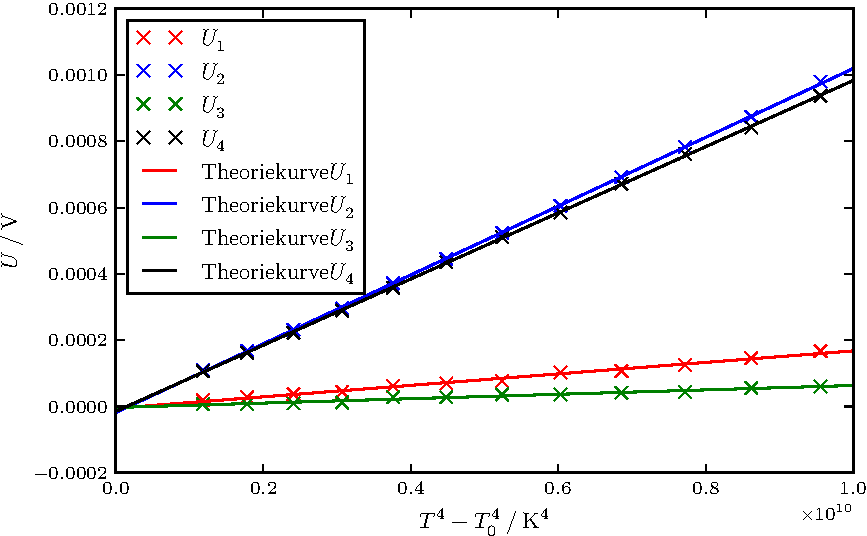
\includegraphics{plot.pdf}
%   \caption{Messdaten und Fitergebnis.}
%   \label{fig:plot}
% \end{figure}
